% A LaTeX (non-official) template for ISAE projects reports
% Copyright (C) 2014 Damien Roque
% Version: 0.2
% Author: Damien Roque <damien.roque_AT_isae.fr>

\documentclass[a4paper,12pt,calibri,oneside,openany]{book}
\usepackage{geometry}
\usepackage[utf8]{inputenc}
\usepackage[T1]{fontenc}
%\usepackage[french]{babel} % If you write in French
\usepackage[english]{babel} % If you write in English
\usepackage{a4wide}
\usepackage{graphicx}
\graphicspath{{images/}}
\usepackage{subfig}
\usepackage{tikz}
\usetikzlibrary{shapes,arrows}
\usepackage{pgfplots}
\pgfplotsset{compat=newest}
\pgfplotsset{plot coordinates/math parser=false}
\newlength\figureheight
\newlength\figurewidth
\pgfkeys{/pgf/number format/.cd,
set decimal separator={,\!},
1000 sep={\,},
}
\usepackage{ifthen}
\usepackage{ifpdf}
\ifpdf
\usepackage[pdftex]{hyperref}
\else
\usepackage{hyperref}
\fi
\usepackage{color}
\usepackage{minted}
\hypersetup{%
colorlinks=true,
linkcolor=black,
citecolor=black,
urlcolor=black}
\usepackage{float}
\renewcommand{\baselinestretch}{1.05}
\usepackage{fancyhdr}
\pagestyle{fancy}
\fancyfoot{}
\fancyhead[LE,RO]{\bfseries\thepage}
\fancyhead[RE]{\bfseries\nouppercase{\leftmark}}
\fancyhead[LO]{\bfseries\nouppercase{\rightmark}}
\setlength{\headheight}{15pt}

\newcommand{\unit}[1]{\ensuremath{\, \mathrm{#1}}}
\let\headruleORIG\headrule
\renewcommand{\headrule}{\color{black} \headruleORIG}
\renewcommand{\headrulewidth}{1.0pt}
\usepackage{colortbl}
\arrayrulecolor{black}

\fancypagestyle{plain}{
  \fancyhead{}
  \fancyfoot[C]{\thepage}
  \renewcommand{\headrulewidth}{0pt}
}

\makeatletter
\def\@textbottom{\vskip \z@ \@plus 1pt}
\let\@texttop\relax
\makeatother

\makeatletter
\def\cleardoublepage{\clearpage\if@twoside \ifodd\c@page\else%
  \hbox{}%
  \thispagestyle{empty}%
  \newpage%
  \if@twocolumn\hbox{}\newpage\fi\fi\fi}
\makeatother

\usepackage{amsthm}
\usepackage{amssymb,amsmath,bbm}
\usepackage{array}
\usepackage{bm}
\usepackage{multirow}
\usepackage[footnote]{acronym}
\usepackage{float}
\usepackage{wasysym}
\usepackage{wrapfig}
\usepackage{url}
\usepackage{eurosym}
\usepackage{array}
\usepackage{xcolor}
\usepackage{supertabular}
%\usepackage{geometry}
\usepackage{pdflscape}
\usepackage{calrsfs}
\usepackage{longtable, booktabs}

\newcommand*{\SET}[1]  {\ensuremath{\mathbf{#1}}}
\newcommand*{\VEC}[1]  {\ensuremath{\boldsymbol{#1}}}
\newcommand*{\FAM}[1]  {\ensuremath{\boldsymbol{#1}}}
\newcommand*{\MAT}[1]  {\ensuremath{\boldsymbol{#1}}}
\newcommand*{\OP}[1]  {\ensuremath{\mathrm{#1}}}
\newcommand*{\NORM}[1]  {\ensuremath{\left\|#1\right\|}}
\newcommand*{\DPR}[2]  {\ensuremath{\left \langle #1,#2 \right \rangle}}
\newcommand*{\calbf}[1]  {\ensuremath{\boldsymbol{\mathcal{#1}}}}
\newcommand*{\shift}[1]  {\ensuremath{\boldsymbol{#1}}}

\newcommand{\eqdef}{\stackrel{\mathrm{def}}{=}}
\newcommand{\argmax}{\operatornamewithlimits{argmax}}
\newcommand{\argmin}{\operatornamewithlimits{argmin}}
\newcommand{\ud}{\, \mathrm{d}}
\newcommand{\vect}{\text{Vect}}
\newcommand{\sinc}{\ensuremath{\mathrm{sinc}}}
\newcommand{\esp}{\ensuremath{\mathbb{E}}}
\newcommand{\hilbert}{\ensuremath{\mathcal{H}}}
\newcommand{\fourier}{\ensuremath{\mathcal{F}}}
\newcommand{\sgn}{\text{sgn}}
\newcommand{\intTT}{\int_{-T}^{T}}
\newcommand{\intT}{\int_{-\frac{T}{2}}^{\frac{T}{2}}}
\newcommand{\intinf}{\int_{-\infty}^{+\infty}}
\newcommand{\Sh}{\ensuremath{\boldsymbol{S}}}
\newcommand{\C}{\SET{C}}
\newcommand{\R}{\SET{R}}
\newcommand{\Z}{\SET{Z}}
\newcommand{\N}{\SET{N}}
\newcommand{\K}{\SET{K}}
\newcommand{\reel}{\mathcal{R}}
\newcommand{\imag}{\mathcal{I}}
\newcommand{\cmnr}{c_{m,n}^\reel}
\newcommand{\cmni}{c_{m,n}^\imag}
\newcommand{\cnr}{c_{n}^\reel}
\newcommand{\cni}{c_{n}^\imag}
\newcommand{\tproto}{g}
\newcommand{\rproto}{\check{g}}
\newcommand{\LR}{\mathcal{L}_2(\SET{R})}
\newcommand{\LZ}{\ell_2(\SET{Z})}
\newcommand{\LZI}[1]{\ell_2(\SET{#1})}
\newcommand{\LZZ}{\ell_2(\SET{Z}^2)}
\newcommand{\diag}{\operatorname{diag}}
\newcommand{\noise}{z}
\newcommand{\Noise}{Z}
\newcommand{\filtnoise}{\zeta}
\newcommand{\tp}{g}
\newcommand{\rp}{\check{g}}
\newcommand{\TP}{G}
\newcommand{\RP}{\check{G}}
\newcommand{\dmin}{d_{\mathrm{min}}}
\newcommand{\Dmin}{D_{\mathrm{min}}}
\newcommand{\Image}{\ensuremath{\text{Im}}}
\newcommand{\Span}{\ensuremath{\text{Span}}}

\newcommand{\anfr}[1]{{\bfseries\underline{#1}}}

\newtheoremstyle{break}
  {11pt}{11pt}%
  {\itshape}{}%
  {\bfseries}{}%
  {\newline}{}%
\theoremstyle{break}

%\theoremstyle{definition}
\newtheorem{definition}{Définition}[chapter]

%\theoremstyle{definition}
\newtheorem{theoreme}{Théorème}[chapter]

%\theoremstyle{remark}
\newtheorem{remarque}{Remarque}[chapter]

%\theoremstyle{plain}
\newtheorem{propriete}{Propriété}[chapter]
\newtheorem{exemple}{Exemple}[chapter]



%\sloppy
\usepackage{wrapfig}
\usepackage{enumitem}
\usepackage{pifont}
\usepackage{makeidx}
\usepackage{setspace}
\makeindex
\usepackage[xindy]{glossaries}
\makeglossaries
%\loadglsentries{glossaire.tex}




\begin{document}

\renewcommand{\bibname}{Bibliographie et Webographie}
%%%%%%%%%%%%%%%%%%
%%% First page %%%
%%%%%%%%%%%%%%%%%%

\begin{titlepage}
\begin{center}


\includegraphics[width=0.6\textwidth]{logohsb}\\[1cm]

%{\large Étudiants ingénieurs en aérospatial}\\[0.5cm]

%{\large DMSP}\\[0.5cm]

% Title
\rule{\linewidth}{0.5mm} \\[0.4cm]
{ \huge \bfseries Satellite Communication\\[0.4cm] }
\rule{\linewidth}{0.5mm} \\[1.cm]
\begin{center}
		Project 3 - POLAR Satellite
\end{center}
% Author and supervisor
\noindent
\begin{minipage}{0.4\textwidth}
  \begin{flushleft} \large
    \emph{Authors :}\\
    Emilio \textbf{\textit{Mitre-Perez}}\\
    Julien \textbf{\textit{Huynh}}\
  \end{flushleft}
\end{minipage}%
\begin{minipage}{0.4\textwidth}
  \begin{flushright} \large
    \emph{Supervising professor :} \\
    Prof. Sören \textit{Peik}\\
  \end{flushright}
\end{minipage}

\vfill



\end{center}
\end{titlepage}

%%%%%%%%%%%%%%%%%%%%%%%%%%%%%
%%% Non-significant pages %%%
%%%%%%%%%%%%%%%%%%%%%%%%%%%%%

\frontmatter

%\chapter*{Remerciements}


\tableofcontents

\mainmatter
\pagestyle{fancy}
%%%%%%%%%%%%%%%%%%%%%%%%%%%%%%%%%%%%%%%%%%%%
%%% Content of the report and references %%%
%%%%%%%%%%%%%%%%%%%%%%%%%%%%%%%%%%%%%%%%%%%%



\chapter{General information}
\section{Polar Satellite}
The POLAR satellite is one of the 4 spacecraft launched for the GGS program (Global Geospace Science) which are part of the six spacecraft of the ISTP program (International Solar Terrestrial Physics). \\
\begin{figure}[h]
	\centering
	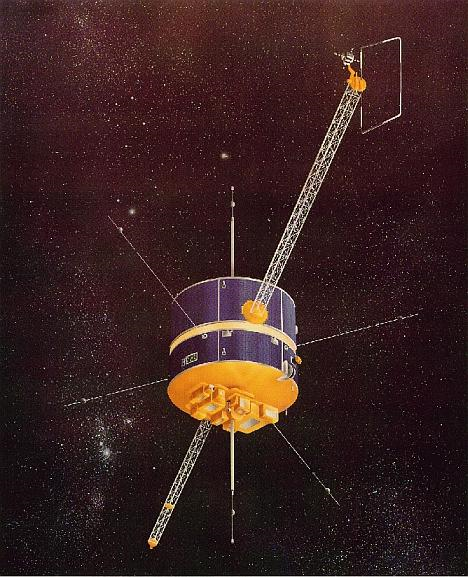
\includegraphics[height=7cm]{polar}
	\caption{Polar Satellite }
\end{figure}
\subsection{Mission and abilities}
POLAR is able to get multi-wavelength vision from the aurora, it measures the plasma entry to the polar magnetosphere as well as the geomagnetic tail, the flow both ways to the ionosphere and the displacement of energy particles into the ionosphere and the higher atmosphere. \\

\subsection{Orbit}
POLAR has a $22h$h and $36$ mins polar orbit with an apogee of $57\ 000$ km and a perigee of $11\ 500$ km. It was launched in 1996 to observe the polar magnetosphere and later was used to observe the equatorial inner. As of $11^{th}$ January $2019$, the two line elements for POLAR (TLE) were :\\

\begin{enumerate}
	\item POLAR,                  
	\item 1 23802U 96013A   20007.96347079  .00000245  00000-0  00000+0 0  9998,
	\item 2 23802  78.7065 252.0668 6485272 288.6366  14.7247  1.29845654114298
\end{enumerate}

\subsection{Technical properties}
The POLAR satellite has a propulsion system and it is designed to have a lifetime of between 3 and 5 years and also has redundant subsystems. POLAR has a cylindrical shape with a $2.8$ m diameter base and $1.25$ m in height (plus $1.25$ m more for the despun platforms), it has solar cells to provide power, weights $1\ 250$ Kg and uses $333$ W of power. The spin rate of the satellite is $10$ RPM around and axis almost normal to the orbital plane. It also has long wire spin-plane antennas, spin-plane appendages to support the sensors and internal booms. The satellite has 2 despun gimbaled instrument platforms, and in the Z axes the booms are deployed.\\

The data is stored in tape recorders on-board and sometimes relayed to the Deep Space network at a maximum speed of 600 kbps and 41.6 kbps in average.\\
 magnetosphere.
 \newpage
\section{Ground Station}
Our ground station will be a small city called Bondy in France, our observer location is :
\begin{enumerate}
	\item Longitude : $2.478680$
	\item Latitude : $48.89976$
\end{enumerate}
\begin{figure}[h]
	\centering
	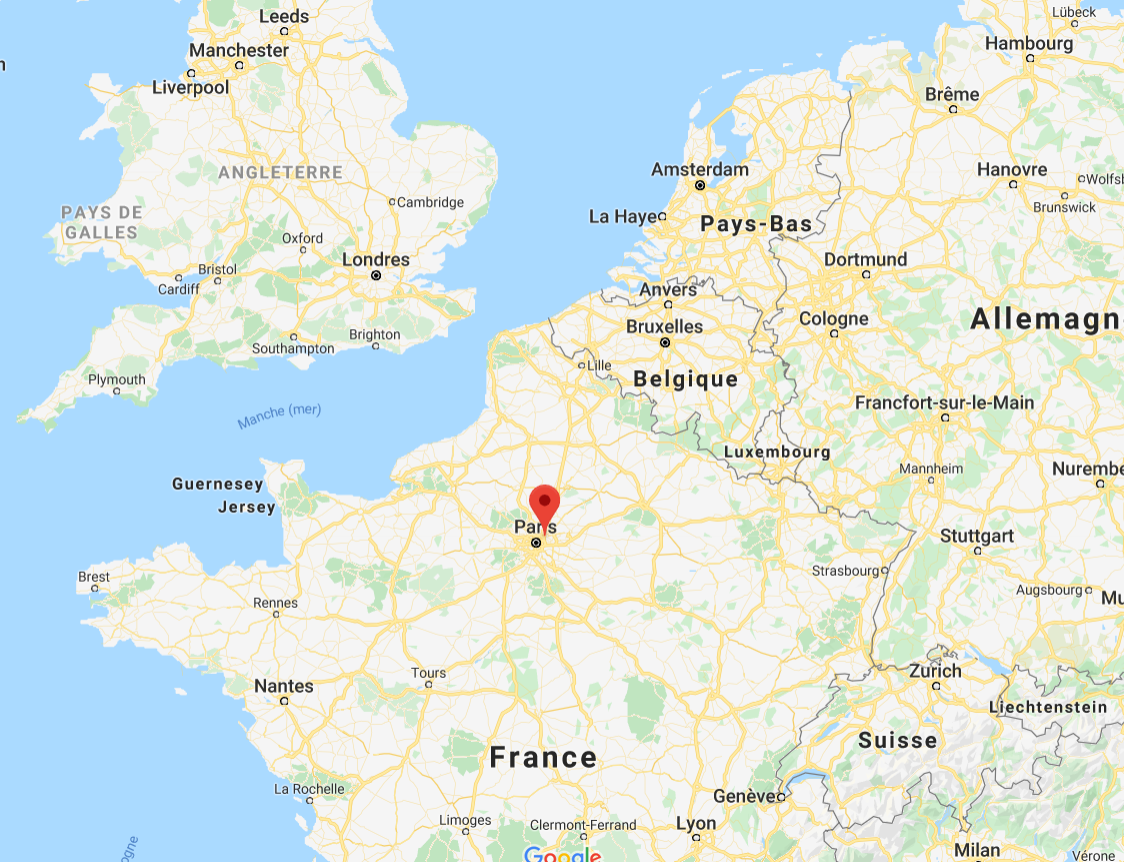
\includegraphics[width=14cm]{bondy}
	\caption{Ground stations }
	\label{Ground Station}
\end{figure}

Our ground station is located approximately $800$ km away from Bremen.
\chapter{Tracking our satellite}
In order to obtain the subpoints of the satellite, we could either use the emphem module or the following formulas : \\
\underline{Latitude $\varphi$} :
$$
\varphi = \arcsin[\sin(i)\cdot \sin(\nu + \omega)]
$$
\underline{Longitude $\lambda$} :
$$
\lambda = \arctan[\tan(\omega + \nu)\cdot \cos(i)] - \bigg[\frac{\Omega_E}n (E-e\cdot\sin(E) - \frac{\Omega_E}{n}\cdot (E_N - e\cdot\sin(E_n))\bigg]
$$

For simplicity reasons, we will use the built-in functions for both the subpoints and the computing of elevation, distance and azimuth with respect to the observer. Those are obtained by the PyEphem package which takes the TLE of the satellite and the ground station longitude and latitude as arguments. The code used is in the Jupyter Notebook.

\newpage
We can then plot the ground track of the POLAR satellite over 5 days starting on $20^{th}$ December $2019$ :

\begin{figure}[H]
	\centering
	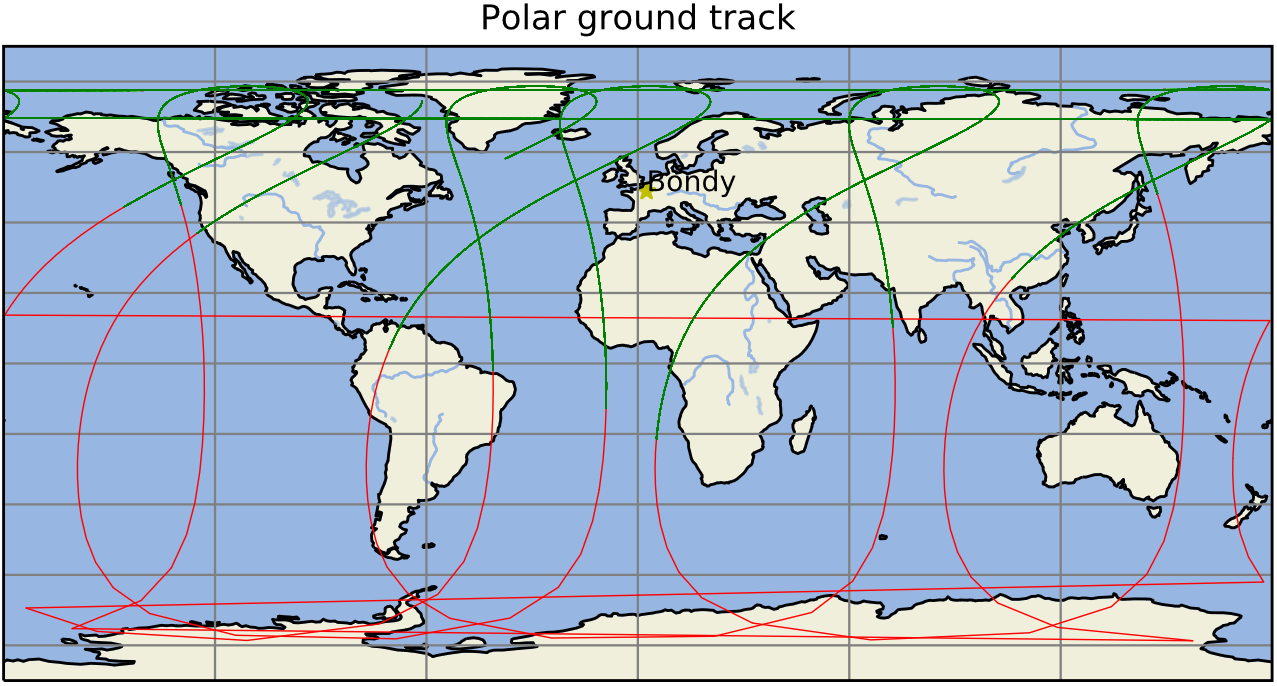
\includegraphics[width=\linewidth]{groundtrack}
	\caption{Ground track of POLAR satellite}
\end{figure}

The red plot is the actual ground track of the satellite and the ground track becomes green when the satellite becomes visible to the ground station. Our visibility condition is that the elevation is at least $5^\circ$.\\

We can then plot the elevation, the distance and the azimuth of the satellite with respect to the ground station over the observation days. Those are also obtained by using the respective PyEphem built-in functions $alt$, $range$ and $az$. For the elevation, the green area is the part in which the satellite is visible to our observer in accordance to the minimal elevation angle.

\begin{figure}[H]
	\centering
	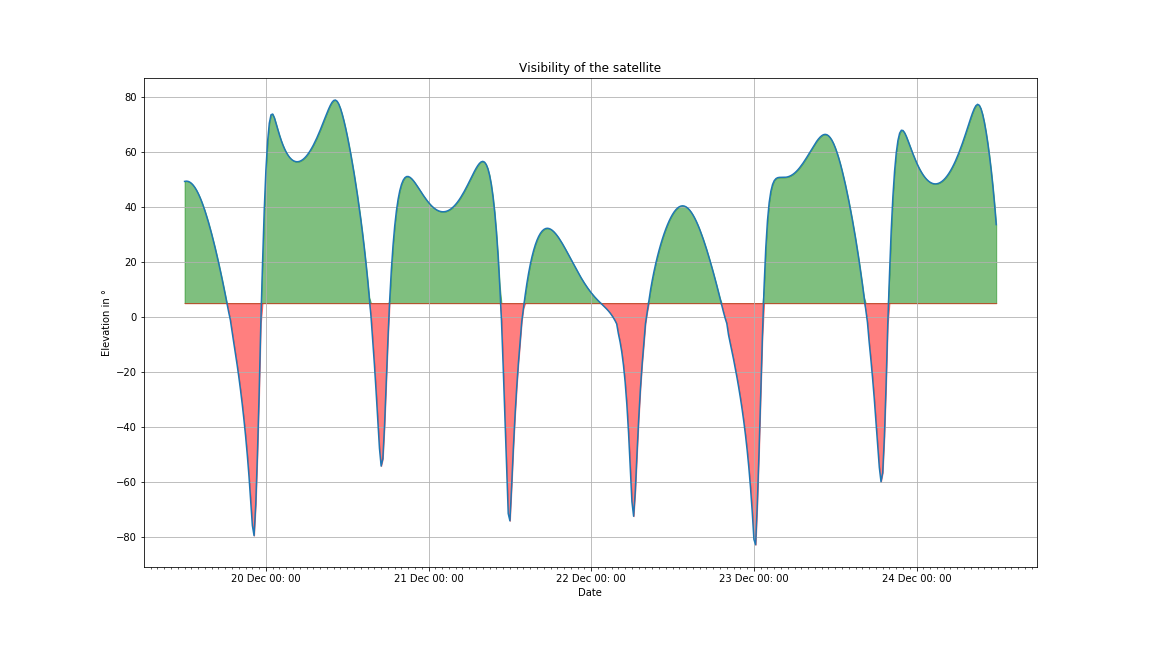
\includegraphics[width=\linewidth]{elevation}
	\caption{Elevation of POLAR satellite with regard to the ground station}
\end{figure}

\begin{figure}[H]
	\centering
	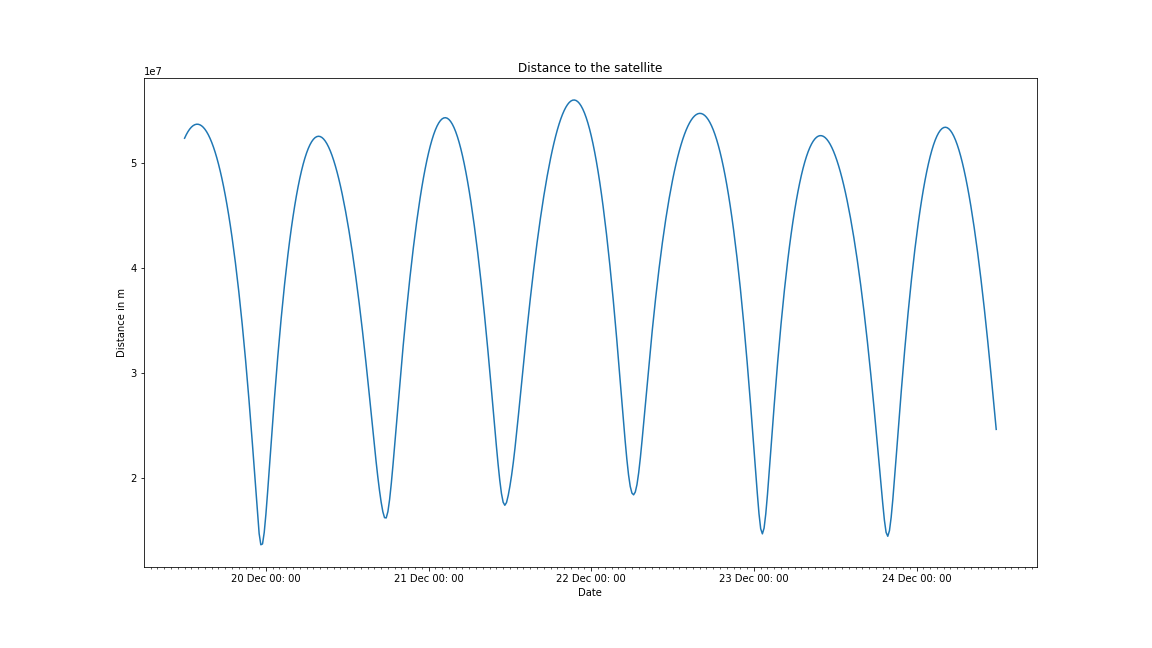
\includegraphics[width=\linewidth]{distance}
	\caption{Distance of POLAR satellite from the ground station}
\end{figure}

\begin{figure}[H]
	\centering
	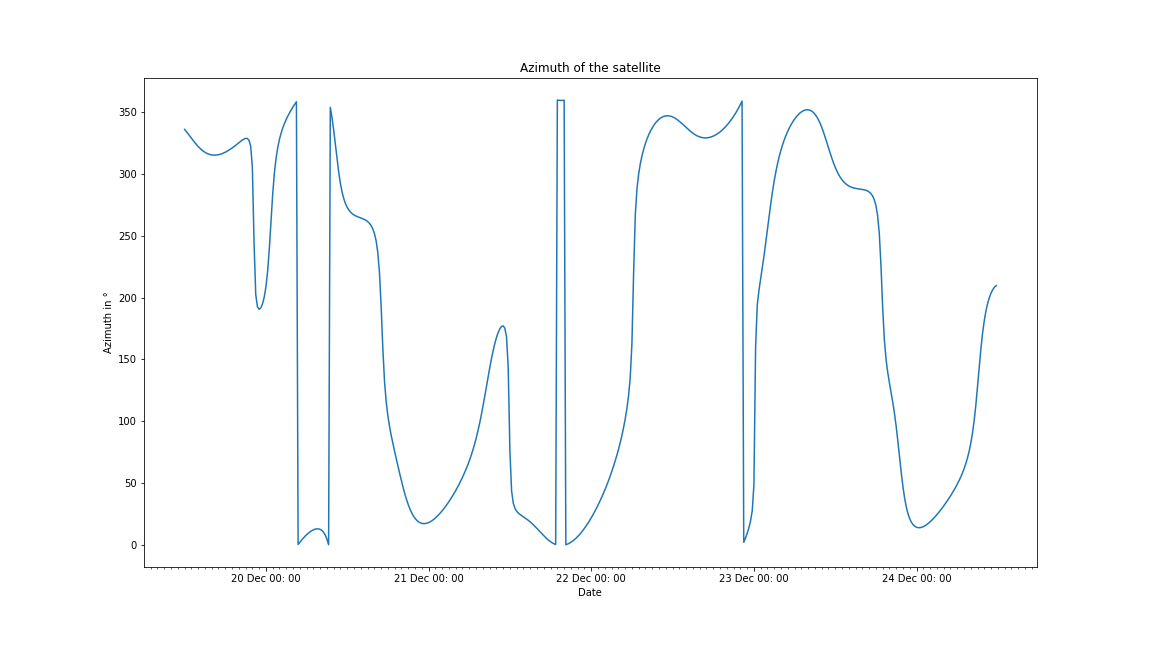
\includegraphics[width=\linewidth]{azimuth}
	\caption{Azimuth of POLAR satellite with regard to the ground station}
\end{figure}

This elevation graph is in accordance with the visible slots on the ground track. When it comes to the distance, it is mainly oscillating between $1\times10^7$ m and $5.6\times 10^7$ m.\\

 The azimuth might look weird at first but it makes sense as the our satellite has a polar orbit with high inclination which then creates such unperiodic function. Moreover, we should keep in mind that those jumps are caused by the fact that the angles are brought back to a $360^\circ$ basis.
\newpage
\section{Connection windows}
\subsection{Largest window}
As we got the information of the orbit of our satellite and its "behavior" with regards to our ground station, we need to find the connection windows we have and make sure that our satellite have the necessary conditions to send us data. The communication windows during our observed timespan are the following :
\begin{enumerate}
	\item Start of window = 2019/12/20 00:00:00\\ End of window = 2019/12/20\\ 06:00:00 Duration = 06:00:00
	\item Start of window = 2019/12/20 11:30:00\\ End of window = 2019/12/21 03:15:00\\ Duration = 15:45:00
	\item Start of window = 2019/12/21 06:15:00\\ End of window = 2019/12/21 22:30:00\\ Duration = 16:15:00
	\item Start of window = 2019/12/22 02:15:00\\ End of window = 2019/12/22 13:15:00\\ Duration = 11:00:00
	\item Start of window = 2019/12/22 20:30:00\\ End of window = 2019/12/23 07:00:00\\ Duration = 10:30:00
	\item Start of window = 2019/12/23 13:30:00\\ End of window = 2019/12/24 04:15:00\\ Duration = 14:45:00
\end{enumerate}

Those windows have been calculated with a large margin as our time resolution was $15$ minutes. We then choose to focus on the largest window which is the $3^{rd}$ one with a duration of approximately $58\ 500$ s.
\newpage
\subsection{Ground track on the largest window}
 We can then plot the ground track of our satellite during that specific window :

\begin{figure}[H]
	\centering
	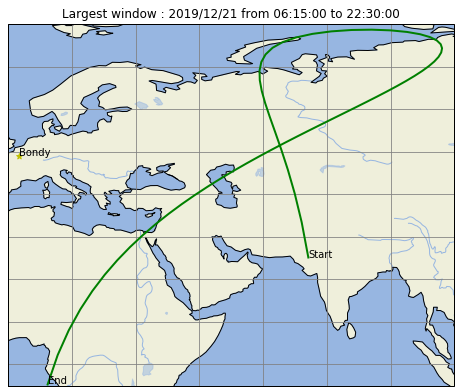
\includegraphics[width=\linewidth]{window}
	\caption{Ground track during the largest window}
\end{figure}
\newpage
\subsection{Distance, azimuth and Doppler shift on the largest window}
We can also take a closer look at the distance from the ground station, the elevation, the azimuth and the Doppler shift on that window :

\begin{figure}[H]
	\centering
	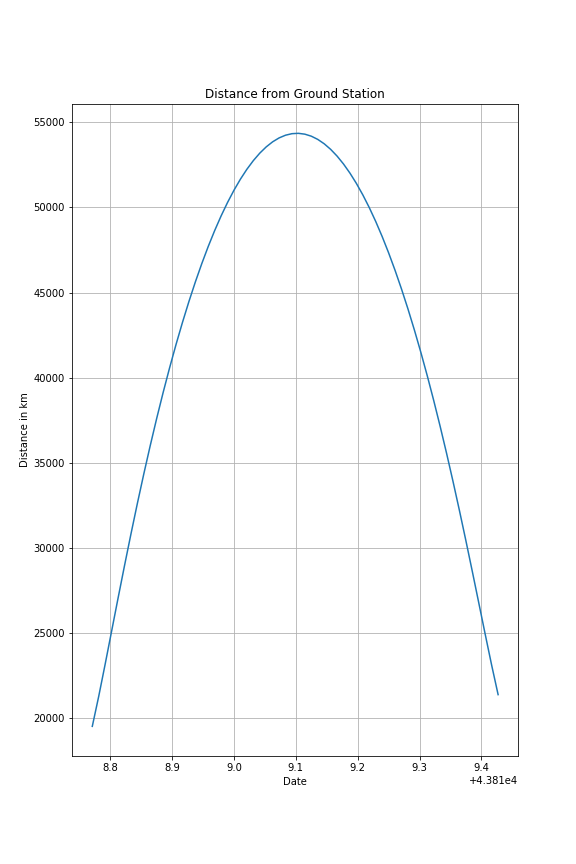
\includegraphics[width=0.7\linewidth]{windowdist}
	\caption{Distance during the largest window}
\end{figure}
\begin{figure}[H]
	\centering
	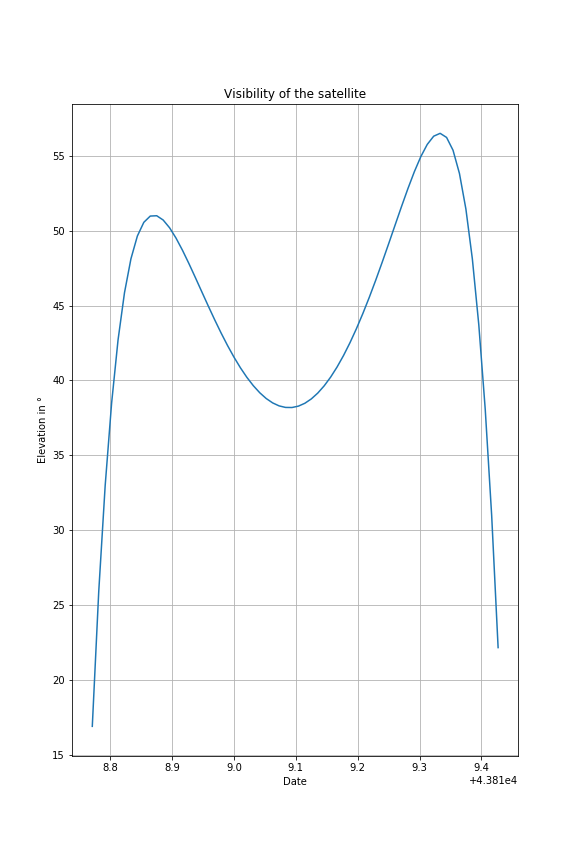
\includegraphics[width=0.7\linewidth]{windowalt}
	\caption{Elevation during the largest window}
\end{figure}
\begin{figure}[H]
	\centering
	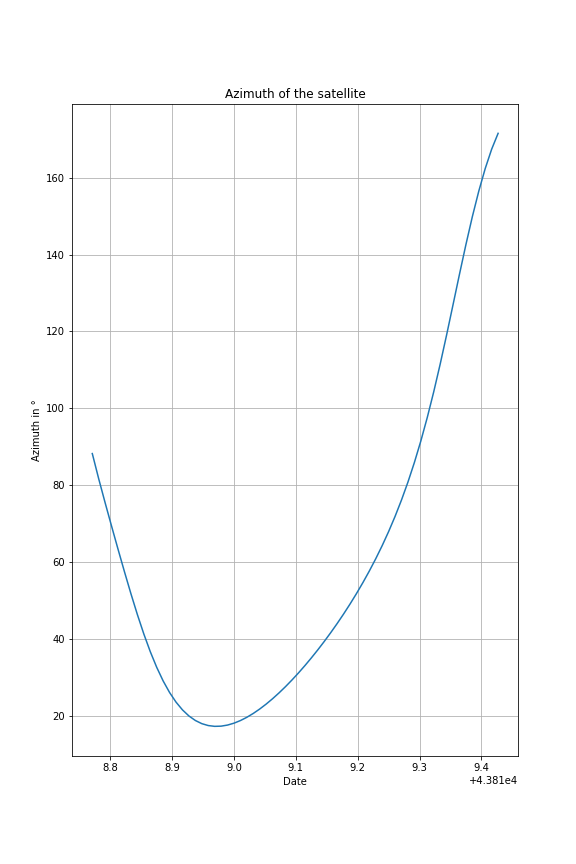
\includegraphics[width=0.7\linewidth]{windowaz}
	\caption{Azimuth during the largest window}
\end{figure}
\subsubsection{Doppler shift}
The Doppler shift can be obtained by :

$$
\Delta_f = \frac{fv_r}{c}
$$
With :
\begin{itemize}
	\item $f$ the frequency of the signal : $8345$ MHz in our case
	\item $v_r$ the range velocity obtained via PyEphem
	\item $c$ the speed of light in vacuum $3\times10^8$ m/s
\end{itemize}
\begin{figure}[H]
	\centering
	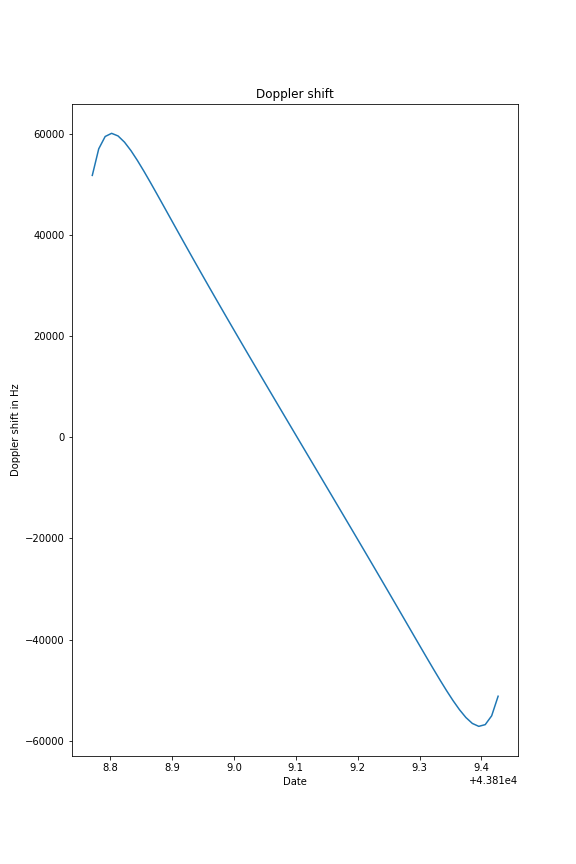
\includegraphics[width=0.6\linewidth]{windowdoppler}
	\caption{Doppler shift during the largest window}
\end{figure}

\chapter{Link and Power budgets}
\section{Link Budget}

	\subsection{Data bit rate and symbol rate}
	
		For the transmission, QPSK (quadrature phase shift keying) modulation is used. The modulation has 4 states so $M=4$ and $m$ can be calculated as $\log_2 M = 2$.
		
		For 16.25 hours of connection time, the required data bit rate $R_{c}$ and symbol rate $R_{a}$ can be obtained by the following expressions:
		
		\begin{equation} \label{eq_rc}
			R_{c}= \dfrac{\# \ of Bits}{T_{con}} = \dfrac{1000 \unit{MByte} \cdot 8 \cdot 10^{8}}{58500 \unit{s}}= 136752.14 \unit{bit/s} 
		\end{equation}
	
		\begin{equation} \label{eq_ra}
			R_{a}= \dfrac{R_{c}}{m} = \dfrac{136752.14 \unit{Bit/s}}{2}= 68376.07 \unit{symbol/s} 
		\end{equation}
	
	\subsection{Required Bandwidth}	
	
		To calculate the bandwidth we will use the following expression:
		
		\begin{equation} \label{eq_ban}
			B= \dfrac{R_{c}}{\Gamma} 
		\end{equation}
	
		We need the value of the roll-off factor which is $\alpha=0.15$ to calculate the spectral efficiency $\Gamma$:
		
		\begin{equation} \label{eq_espectral_eff}
			\Gamma= \dfrac{m}{1+\alpha} = \dfrac{2}{1+0.15} =  1.74
		\end{equation}
		
		And therefore, going back to the equation \ref{eq_ban} the bandwidth value is:
		
		\begin{equation} \label{eq_ban2}
			B= \dfrac{136752.14}{1.74} = 7.86 \cdot 10^{-4} \unit{Hz}
		\end{equation}
	
	\subsection{Required SNR}
	
		For the required BER of $10^{-6}$ and a QPSK modulation scheme, we will use the graph in Figure \ref{graf_BER} to obtain the Energy per bit per noise ratio $\left(\dfrac{E_{c}}{N_{o}}\right)$ and we get a value of $\dfrac{E_{c}}{N_{o}}\approx10.5 \unit{dB}$
	
		\begin{figure}[h]
			\centering
			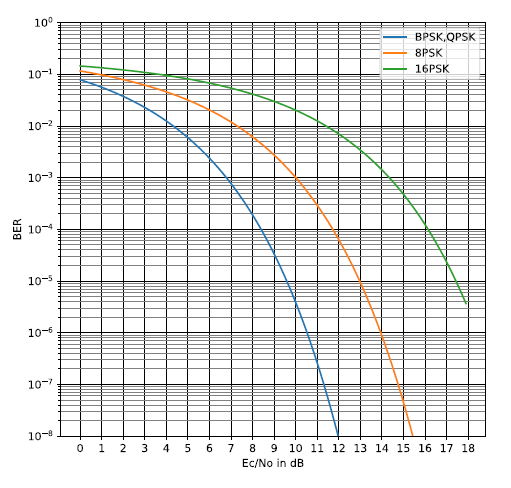
\includegraphics[width=14cm]{graph_BER}
			\caption{Bit Error Ratios for different Modulation Schemes }
			\label{graf_BER}
		\end{figure}
	
		Once we have the $\dfrac{E_{c}}{N_{o}}$ we can proceed to calculate the SNR:
		
		\begin{equation} \label{eq_snr}
			SNR = \dfrac{R_{c} \cdot \dfrac{E_{c}} {N_{o}}}{B} = \dfrac{136752.14 \cdot 10.5} {7.86 \cdot 10^{-4}} = 19,51
		\end{equation}
		
	\subsection{Receiver and noise}	
		
		 To calculate the total received noise at the antenna of the ground station $N_{i}$ we can use the following expression: 
		 
		 \begin{equation} \label{eq_ni}
		 	N_{i} = k \cdot T_{a} \cdot B
		 \end{equation}
	
		In which the $k$ is the Bolzmann constant with a value of $ 1.38 \cdot 10^{-23} \unit{J/K}$, $B$ is the previously calculated bandwidth and $T_{a}$ is the antenna noise temperature, which can be found in the graph of Figure \ref{graph_TA}.
		
		\begin{figure}[h]
			\centering
			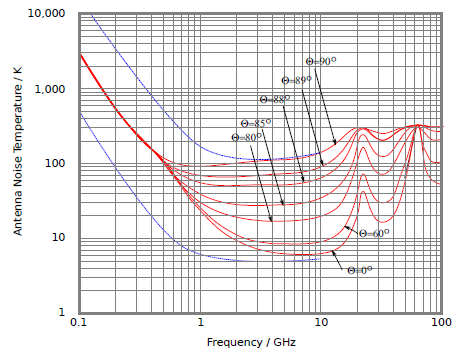
\includegraphics[width=14cm]{graph_TA}
			\caption{Antenna noise temperature $T_{a}$ as a function of the Zenith angle and the frequency.}
			\label{graf_TA}
		\end{figure}
		
		
		To calculate the $T_{a}$ we will take the worst case scenario under consideration, which is for an elevation of $5^{\circ}$ (Zenith Angle $\Theta = 85^{\circ}$). In this case we get a $T_{a} \approx 30.5 \unit{K} $
	
		Now that we have calculated all the values we can put them back in Equation \ref{eq_ni}:
	
		\begin{equation} \label{eq_ni2}
			N_{i} = 1.38 \cdot 10^{-23} \cdot 30.5 \cdot 7.86 \cdot 10^{-4} = 4.21 \cdot 10^{-17} \unit{W}
		\end{equation}
	
		To obtain the input noise $N_{o}$ we will use the following calculation:
		
		\begin{equation} \label{eq_no}
			N_{o} = k \cdot \left(T_{a} + T{e} \right) \cdot B \cdot G_{r} 
		\end{equation}
	
		In which $k$ is the the Bolzmann constant, $T_{a}$ is the previously calculated antenna noise temperature, $T_{e}$ is the equivalent noise temperature, $B$ is the Bandwidth and $G_{r}$ is the gain of the receiver in the ground station. 
		
		To calculate the equivalent noise temperature $T_{e}$ we need the noise figure, which is given as $F=2 \unit{dB}$ and the initial temperature $T_{0}$ which is set at 290 K:
		
		\begin{equation} \label{eq_te}
			T_{e} = (F - 1) \cdot T_{0} = 169.62 \unit{K} 
		\end{equation}
	 	
	 	With all the parameters from Equation \ref{eq_no} known, besides the  gain of the receiver in the ground station which is set to a design value of $G_{r}= 100000$, we can calculate the $N_{o}$:
	 	
	 	\begin{equation} \label{eq_no2}
	 		N_{o} = 1.38 \cdot 10^{-23} \cdot \left(30.5 + 169.62 \right) \cdot 7.86 \cdot 10^{4} \cdot 100000 = 2.76 \cdot 10^{-11} \unit{W}
	 	\end{equation}
	 		
	\subsection{Required signal powers}
	
		To calculate the required signal power $S_{o}$ we use the following equation:
	
		\begin{equation} \label{eq_so}
			S_{o} = SNR \cdot N_{0} = 19,51 \cdot 2.76 \cdot 10^{-11} = 5,39 \cdot 10^{-10}  \unit{W}
		\end{equation}
	
		And to obtain the input signal power $S_{i}$ we will use the receiver gain that we assume before to be 100000 W (or 60 dB):
		
		\begin{equation} \label{eq_si}
			S_{i} = \dfrac{S_{0}}{G_{r}}= \dfrac{5,39 \cdot 10^{-10}}{100000} = 5,39 \cdot 10^{-15}  \unit{W}
		\end{equation}		
	
	\subsection{Required EIRP in worst case scenario}
	
		To calculate the EIRP for the worst case scenario with an elevation of 5$^{\circ}$ we can use the following formula:
		
		\begin{equation} \label{eq_eirp}
		\begin{split}
			EIRP = SNR \cdot &L_{p} \cdot k \cdot B \cdot \dfrac{T_{a}+T_{e}}{G_{a}} = \\
			19.51  \cdot 3.84 \cdot 10^{20} \cdot 1.38 \cdot 10^{-23} \cdot &100000 \cdot \dfrac{30.5+169.61}{4.39 \cdot 10^{3}} = 451.31	 \unit{W}
		\end{split}
		\end{equation}
	
	\subsection{Design a transmitter with 30\% efficiency and a matching dish antenna}
	
		Finally we ought to design a transmitter with a 30\% efficiency and its antenna. For the transmitter we set a design value of 25 W. The first thing we have to calculate is the gain of the transmitter $G_{t}$:
		
		\begin{equation} \label{eq_gt}
			G_{t} = \dfrac{EIRP}{P_{t}}= \dfrac{451.31}{25} = 18.05
		\end{equation}
	
		Now that we have the gain of the transmitter, we will proceed to define the size of the antenna. For knowing its diameter $D$, we will have to know the phisical area of the antenna $A_{phy}$, and for that the effective area of the antenna $A_{eff}$:
		
		\begin{equation} \label{eq_aeff}
			A_{eff} = \dfrac{G_{t} \cdot \lambda^{2}} {4 \cdot \pi }
		\end{equation}
	
		Where lambda $\lambda$ is the wavelenght and can be calculated with the frequency $f$ and the speed of light $c$:
		
		\begin{equation} \label{eq_lambda}
			\lambda = \dfrac{c} {f}= \dfrac{2.998 \cdot 10^{8}} {8.35 \cdot 10^{9}} = 3.59 \cdot 10^{-2} \unit{m}
		\end{equation}
	
		Going back to the Equation \ref{eq_aeff}:
		
		\begin{equation} \label{eq_aeff2}
			A_{eff} = \dfrac{{18.05} \cdot (3.59 \cdot 10^{-2})^{2}} {4 \cdot \pi } =  1.86 \cdot 10^{-3} \unit{m^{2}}
		\end{equation}
	
		\begin{equation} \label{eq_aphy}
			A_{phy} = \dfrac{A_{eff}} {\eta_{t}} = 
			\dfrac{1.86 \cdot 10^{-3}} {0.3}=
			6.18 \cdot 10^{-3} \unit{m^{2}}
		\end{equation}
		
		\begin{equation} \label{eq_d}
			D = 2 \cdot \sqrt{\dfrac{A_{phy}}{\pi}} =
			2 \cdot \sqrt{\dfrac{6.18 \cdot 10^{-3}}{\pi}} = 8.87  \unit{m}
		\end{equation}
	
	\section{Summary table}	

		\begin{center}
			\begin{tabular}{ | l | l | l | p{1.5cm} |}
				\hline
				Description & Quantity & Value & Unit \\ \hline
				Frequency & f  & $8,35*10^{9}$ & Hz \\ \hline
				Tx-Power & Pt & 25 & W
				\\ \hline
				Tx-Antenna gain & Gt & $18.1$ & 
				\\ \hline
				Tx-EIRP & EIRP & $4.51*10^{2}$ & W
				\\ \hline
				Tx Dish Diameter & D & $8.87*10^{-2}$ & m
				\\ \hline
				Mod. Scheme & QPSK &  & 
				\\ \hline
				Bandwidth & B & $7.86*10^{4}$ & Hz
				\\ \hline
				Max. Distance to Ground & r & $5.60*10^{7}$ & m
				\\ \hline
				Rx-Antenna Gain & Gr & $10^{5}$ & 
				\\ \hline
				Rx-Dish Diameter & D & 1 & m
				\\ \hline
				G/T of Rx & G/T & 22.9 & $K^{-1}$
				\\ \hline
				Received Power & Prec & $5.39*10^{-15}$ & W
				\\ \hline
				
						\end{tabular}
					\end{center}
				
\newpage
\section{Power Budget}
	\subsection{Battery capacity and solar cell area}
	
		To calculate the battery capacity we will need the power consumption $P_{tot}$ and the time that the satellite is in the shadow $t_{eclipse} = 3 hours$. For the power we have assumed that the platform requires 500 W when it is in the sun and 100 W when it is in the shadow.
		
		\begin{equation} \label{eq_cb}
			CB = \dfrac{P_{tot}}{t_{eclipse}} =
			\dfrac{P_{psun} +  P_{pshadow} + P_{t} }{t_{eclipse}}=
			\dfrac{500 +  100 + 25 } {3} = 208.33 \unit{Wh}
		\end{equation}
		
		For the required solar cell area $A_{sol}$ we will need the Irradiance $M_{sol}$ which has a value of $1367 \unit{W/m^{2}}$, the efficiency of the cell $\eta_{cell}$ which we set to 0.15 and the power required by the satellite when it is in the sun $P_{sol}$.
		
		To calculate the $P_{sol}$(Equation \ref{eq_psol}) we need to know first the power that it consumes to charge the battery $P_{charging}$, for which we need the period of the elipse $T_{elipse}$, the time on the shadow $t_{eclipse}$ and the efficiency of the battery $\eta_{bat}$, as well as the already calculated battery capacity $CB$.
		
		\begin{equation} \label{eq_pcharging}
			P_{charging} = \dfrac{CB}{\dfrac{T_{elipse}-t_{eclipse}} {\eta{bat}}	} =
			\dfrac{208.33}{\dfrac{18.5-3}{0.8}	} = 16.80 \unit{W}
		\end{equation}
		
		\begin{equation} \label{eq_psol}
			P_{sol} = P_{charging} + P_{psun} + P_{t}= 
			16.80 + 500 + 25= 541.80 \unit{W}
		\end{equation}
		
		Now that we have all the values we can calculate the required solar cell area $A_{sol}$:
		
		\begin{equation} \label{eq_asol}
			A_{sol} = \dfrac{P_{sol}}{M_{sol} \cdot \eta_{cell}}= \dfrac{541.80}{1367 \cdot 0.15}=  2.64 \unit{m^{2}}
		\end{equation}
		
	
	





%\glsaddall
%\printglossaries

%\nocite{*}

	
%	\bibliographystyle{plain} % Le style est mis entre accolades.
%	\bibliography{references} % mon fichier de base de données s'appelle bibli.bib

%\printbibliography



%\include{lexique_an_fr}
\listoffigures

%\listoftables
%\nopagebreak
%\include{annexes}

%\printindex

\end{document}
